\section{Question 4}
\subsection{Part 1}
Consider the following BN for the given model: 
\begin{figure}[H]
    \centering
    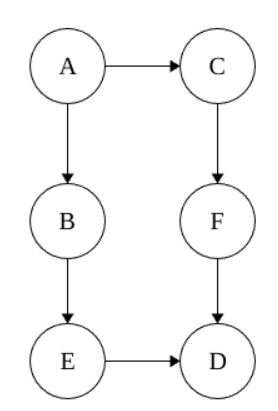
\includegraphics[width=0.3\textwidth]{../images/BN_Q4.png}
\end{figure}
Since P factorizes over G, G is an I-map for P. Since $I(G) \subseteq I(P)$, the conditional independence $F \independent B | A$, which holds in this graph, holds in P as well.
\subsection{Part 2}
We cannot guarantee that C is independent of E. In this very graph, C-A-B-E is an active path from C to E given no observed variables.
We at the same time cannot guarantee that C is dependent on E. Consider the graph below, which satisfies all the conditional independencies satisfied in P and some more.
\begin{figure}[H]
    \centering
    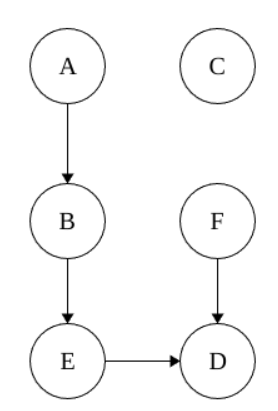
\includegraphics[width=0.3\textwidth]{../images/BN_Q4_2.png}
\end{figure}
